\section{Introducción}
\subsection{Evolución de la Concurrencia en Java}
\begin{frame}
\begin{center}
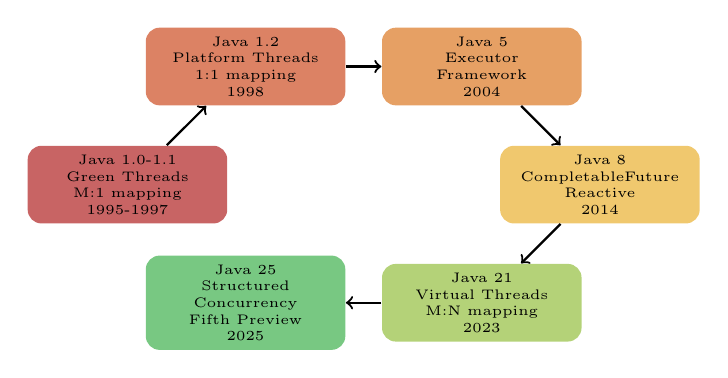
\begin{tikzpicture}[
    box/.style={rectangle, text width=2.3cm, align=center,
                font=\tiny, rounded corners=5pt},
    box1/.style={box, fill={rgb,255: red,200; green,100; blue,100}},
    box2/.style={box, fill={rgb,255: red,220; green,130; blue,100}},
    box3/.style={box, fill={rgb,255: red,230; green,160; blue,100}},
    box4/.style={box, fill={rgb,255: red,240; green,200; blue,110}},
    box5/.style={box, fill={rgb,255: red,180; green,210; blue,120}},
    box6/.style={box, fill={rgb,255: red,120; green,200; blue,130}}
]
\node (green) [box1] at (-3, 0) {Java 1.0-1.1\\Green Threads\\M:1 mapping\\1995-1997};
\node (platform) [box2] at (-1.5, 1.5) {Java 1.2\\Platform Threads\\1:1 mapping\\1998};
\node (executor) [box3] at (1.5, 1.5) {Java 5\\Executor\\Framework\\2004};
\node (reactive) [box4] at (3, 0) {Java 8\\CompletableFuture\\Reactive\\2014};
\node (virtual) [box5] at (1.5, -1.5) {Java 21\\Virtual Threads\\M:N mapping\\2023};
\node (structured) [box6] at (-1.5, -1.5) {Java 25\\Structured Concurrency\\Fifth Preview\\2025};

\draw [->, thick] (green) -- (platform);
\draw [->, thick] (platform) -- (executor);
\draw [->, thick] (executor) -- (reactive);
\draw [->, thick] (reactive) -- (virtual);
\draw [->, thick] (virtual) -- (structured);
\end{tikzpicture}
\end{center}
\begin{alertblock}{Estado en Java 25}
\begin{itemize}
\item Virtual Threads: \textbf{Estable} (desde Java 21)
\item Scoped Values: \textbf{Estable} desde Java 25 ~\cite{JEP506}
\item Structured Concurrency: \textbf{Quinta Preview} en Java 25 ~\cite{JEP505}
\end{itemize}
\end{alertblock}
\end{frame}
